% answers.tex —— 1961 年·全国卷 · 参考答案与详细解析片段
% 由 tools/generate_projects.py 依来源总账自 1961/1961_数学真题_试题.md + 1961/1961_数学真题_解析正文.md + 1961/1961_数学真题_答案要点.md 生成，勿手改（改源 MD 后重跑）


\gkpart{一、小题}

\begin{answer}
\gksolhead{1}{}

\textbf{题目}：

（1）求 $(2-x)^{10}$ 展开式里 $x^7$ 的系数。

\Needspace{4\baselineskip}
\textbf{解析}

\Needspace{5\baselineskip}
展开式一般项为
\nopagebreak[4]
\[
\binom{10}{r}2^{10-r}(-x)^r.
\]
\Needspace{5\baselineskip}
含 $x^7$ 的项取 $r=7$，所以其系数为
\nopagebreak[4]
\[
\binom{10}{7}2^3(-1)^7
=-\binom{10}{3}\cdot8
=-960.
\]

\gkanswer{答案：$-960$。}

\end{answer}
\begin{answer}
\gksolhead{2}{}

\textbf{题目}：

\Needspace{5\baselineskip}
（2）解方程：
\nopagebreak[4]
\[
2\lg x=\lg(x+12)
\]
（注：$\lg$ 是以 10 为底的对数的符号。）

\Needspace{4\baselineskip}
\textbf{解析}

\Needspace{5\baselineskip}
由对数的定义，必须有 $x>0$，且
\nopagebreak[4]
\[
2\lg x=\lg x^2=\lg(x+12).
\]
\Needspace{5\baselineskip}
因此
\nopagebreak[4]
\[
x^2=x+12,
\qquad x^2-x-12=0,
\qquad (x-4)(x+3)=0.
\]
候选值为 $x=4$ 或 $x=-3$。由于 $\lg x$ 要求 $x>0$，舍去 $-3$，故 $x=4$。

\gkanswer{答案：$x=4$。}

\end{answer}
\begin{answer}
\gksolhead{3}{}

\textbf{题目}：

\Needspace{5\baselineskip}
（3）求函数
\nopagebreak[4]
\[
y=\frac{\sqrt{x-1}}{x-5}
\]
的自变量 $x$ 的允许值的范围。

\Needspace{4\baselineskip}
\textbf{解析}

\Needspace{5\baselineskip}
根式有意义要求
\nopagebreak[4]
\[
x-1\ge0,
\qquad x\ge1.
\]
同时分母不能为零，故 $x-5\ne0$，即 $x\ne5$。所以允许值范围为 $x\ge1$ 且 $x\ne5$。

\gkanswer{答案：$x\ge1$ 且 $x\ne5$。}

\end{answer}
\begin{answer}
\gksolhead{4}{}

\textbf{题目}：

\Needspace{5\baselineskip}
（4）求
\nopagebreak[4]
\[
\sin\frac{\pi}{12}\sin\frac{5\pi}{12}
\]
的值。

\Needspace{4\baselineskip}
\textbf{解析}

\Needspace{5\baselineskip}
利用积化和差公式，
\nopagebreak[4]
\[
\sin\frac\pi{12}\sin\frac{5\pi}{12}
=\frac12\left(\cos\frac\pi3-\cos\frac\pi2\right)
=\frac12\left(\frac12-0\right)=\frac14.
\]

\gkanswer{答案：$\dfrac14$。}

\end{answer}
\begin{answer}
\gksolhead{5}{}

\textbf{题目}：

（5）一个水平放着的圆柱形排水管，内半径是 $12$ 厘米。排水管的圆截面上被水淹没部分的弧含有 $150^\circ$（如图）。求这个截面上有水部分的面积。（取 $\pi=3.14$。）
\nopagebreak[4]
\begin{center}% 1961 年全国卷第 5 题：排水管圆截面中的水弓形。
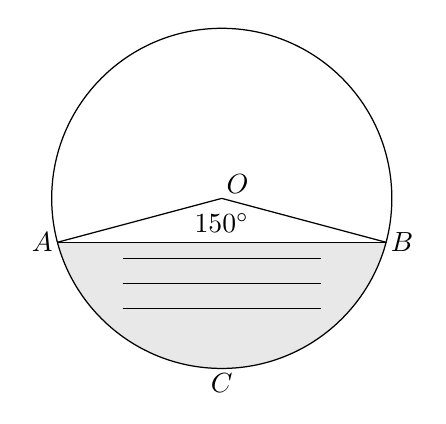
\begin{tikzpicture}[scale=0.9, line width=0.45pt,
  every node/.style={inner sep=1.5pt}]
  \coordinate (O) at (0,0);
  \coordinate (A) at (-2.32,-0.62);
  \coordinate (B) at (2.32,-0.62);
  \fill[gray!18] (A) arc (195:345:2.4) -- cycle;
  \draw (O) circle (2.4);
  \draw (A)--(B);
  \draw (O)--(A) (O)--(B);
  \foreach \y in {-1.55,-1.2,-0.85} {
    \draw (-1.4,\y)--(1.4,\y);
  }
  \node[anchor=east] at (A) {$A$};
  \node[anchor=west] at (B) {$B$};
  \node[anchor=south west] at (O) {$O$};
  \node at (0,-0.35) {$150^\circ$};
  \node[anchor=north] at (0,-2.4) {$C$};
\end{tikzpicture}
\end{center}
\nopagebreak[4]
\Needspace{4\baselineskip}
\textbf{解析}

\Needspace{5\baselineskip}
设圆截面圆心为 $O$，半径 $r=12$ 厘米，水面弦为 $AB$，水面以下的圆弧 $ACB$ 所对圆心角为 $150^\circ$。扇形 $O$—$ACB$ 的圆心角为 $150^\circ$，弧长为
\nopagebreak[4]
\[
12\times\frac{5\pi}{6}=10\pi.
\]
\Needspace{5\baselineskip}
所以扇形面积为
\nopagebreak[4]
\[
\frac12\times12\times10\pi=60\pi.
\]
\Needspace{5\baselineskip}
三角形 $OAB$ 的面积为
\nopagebreak[4]
\[
\frac12\times12^2\sin150^\circ=36.
\]
\Needspace{5\baselineskip}
水淹没的弓形面积为
\nopagebreak[4]
\[
60\pi-36=60\times3.14-36=152.4\text{ 平方厘米}.
\]

\gkanswer{答案：$152.4$ 平方厘米。}

\end{answer}
\begin{answer}
\gksolhead{6}{}

\textbf{题目}：

（6）已知 $\triangle ABC$ 的一边 $BC$ 在平面 $N$ 内，$\triangle ABC$ 所在的平面与平面 $N$ 组成二面角 $\alpha$（$\alpha<90^\circ$）。从 $A$ 点作平面 $N$ 的垂线 $AA'$，$A'$ 是垂足。设 $\triangle ABC$ 的面积是 $S$，求证 $\triangle A'BC$ 的面积是 $S\cos\alpha$。

\Needspace{4\baselineskip}
\textbf{解析}
\nopagebreak[4]
\begin{center}% 1961 年全国卷第 6 题：三角形到平面的正投影。
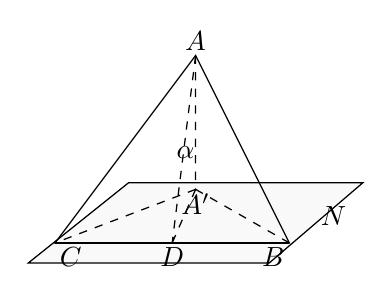
\begin{tikzpicture}[scale=0.85, line width=0.45pt,
  every node/.style={inner sep=1.5pt}]
  \coordinate (C) at (-2.0,-0.8);
  \coordinate (B) at (1.5,-0.8);
  \coordinate (A) at (0.1,2.0);
  \coordinate (Ap) at (0.1,0.0);
  \coordinate (D) at (-0.25,-0.8);
  \draw[fill=gray!5] (-2.4,-1.1)--(1.2,-1.1)--(2.6,0.1)--(-0.9,0.1)--cycle;
  \draw (A)--(B)--(C)--cycle;
  \draw[dashed] (A)--(Ap) (Ap)--(B) (Ap)--(C);
  \draw[dashed] (A)--(D) (Ap)--(D);
  \draw (C)--(B);
  \node[anchor=south] at (A) {$A$};
  \node[anchor=north] at (Ap) {$A'$};
  \node[anchor=north east] at (B) {$B$};
  \node[anchor=north west] at (C) {$C$};
  \node[anchor=north] at (D) {$D$};
  \node[anchor=west] at (1.9,-0.4) {$N$};
  \node at (-0.05,0.55) {$\alpha$};
\end{tikzpicture}
\end{center}
\nopagebreak[4]
\Needspace{5\baselineskip}
作 $AD\perp BC$ 于 $D$，连接 $A'D$。由于 $A'$、$D$ 都在平面 $N$ 内且 $AD\perp BC$，$A'D$ 是 $AD$ 在平面 $N$ 上的射影，且 $A'D\perp BC$。二面角的平面角满足
\nopagebreak[4]
\[
\angle ADA'=\alpha.
\]
\Needspace{5\baselineskip}
在直角三角形 $AA'D$ 中，
\nopagebreak[4]
\[
A'D=AD\cos\alpha.
\]
\Needspace{5\baselineskip}
于是
\nopagebreak[4]
\[
[\triangle A'BC]=\frac12BC\cdot A'D
=\frac12BC\cdot AD\cos\alpha
=[\triangle ABC]\cos\alpha
=S\cos\alpha.
\]

\gkanswer{答案：$\triangle A'BC$ 的面积为 $S\cos\alpha$。}

\end{answer}
\gkpart{二、大题}

\begin{answer}
\gksolhead{7}{}

\textbf{题目}：

一个机器制造厂的三年生产计划，每年比上一年增产机器的台数相同。如果第三年比原计划多生产 1 千台，那么每年比上一年增长的百分数就相同，而且第三年生产的台数恰等于原计划三年生产总台数的一半。原计划每年各生产机器多少台？

\Needspace{4\baselineskip}
\textbf{解析}

\Needspace{5\baselineskip}
以千台为单位，设原计划第一、二、三年分别生产 $x$、$x+y$、$x+2y$ 千台。第三年实际生产 $x+2y+1$ 千台，增长百分数相同给出
\nopagebreak[4]
\[
\frac{(x+y)-x}{x}
=\frac{(x+2y+1)-(x+y)}{x+y}.
\]
\Needspace{5\baselineskip}
又由第三年实际产量是原计划总产量的一半，
\nopagebreak[4]
\[
x+2y+1=\frac12\bigl[x+(x+y)+(x+2y)\bigr].
\]
\Needspace{5\baselineskip}
化简得
\nopagebreak[4]
\[
y^2-x=0,
\qquad x-y-2=0.
\]
解得 $(x,y)=(4,2)$ 或 $(1,-1)$。产量增长量取正值，舍去后一组，故三年产量为 $4$、$6$、$8$ 千台。

\gkanswer{答案：原计划第一、二、三年各生产 $4$ 千台、$6$ 千台、$8$ 千台。}

\end{answer}
\begin{answer}
\gksolhead{8}{}

\textbf{题目}：

有一块圆环形的铁皮，它的内半径是 $45$ 厘米，外半径是 $75$ 厘米。用它的五分之一（如图中的阴影部分），作圆台形水桶的侧面。这个水桶的容积是多少立方厘米？
\nopagebreak[4]
\begin{center}% 1961 年全国卷第 8 题：圆环铁皮的五分之一扇形。
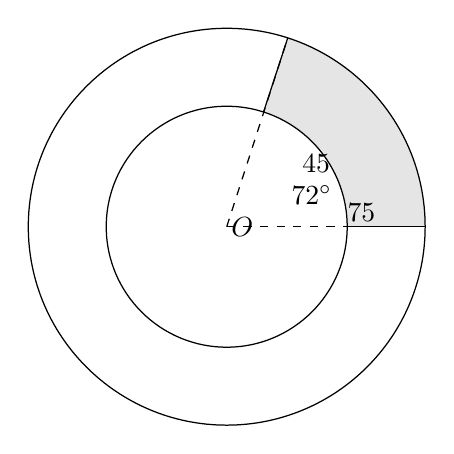
\begin{tikzpicture}[scale=0.9, line width=0.45pt,
  every node/.style={inner sep=1.5pt}]
  \coordinate (O) at (0,0);
  \fill[gray!20] (2.8,0) arc (0:72:2.8)
    -- (0.52,1.62) arc (72:0:1.7) -- cycle;
  \draw (O) circle (2.8);
  \draw (O) circle (1.7);
  \draw (2.8,0)--(1.7,0);
  \draw (0.86,2.66)--(0.52,1.62);
  \draw[dashed] (O)--(2.8,0);
  \draw[dashed] (O)--(0.86,2.66);
  \node[anchor=west] at (O) {$O$};
  \node[anchor=south] at (1.9,0) {$75$};
  \node[anchor=south west] at (1.0,0.7) {$45$};
  \node at (1.2,0.45) {$72^\circ$};
\end{tikzpicture}
\end{center}
\nopagebreak[4]
\Needspace{4\baselineskip}
\textbf{解析}

\Needspace{5\baselineskip}
圆环铁皮的五分之一卷成圆台侧面，因此圆台上、下底半径分别为
\nopagebreak[4]
\[
R=\frac{75}{5}=15\text{ 厘米},
\qquad r=\frac{45}{5}=9\text{ 厘米}.
\]
\Needspace{5\baselineskip}
圆台的母线长为
\nopagebreak[4]
\[
l=75-45=30\text{ 厘米}.
\]
\Needspace{5\baselineskip}
圆台高为
\nopagebreak[4]
\[
h=\sqrt{l^2-(R-r)^2}
=\sqrt{30^2-6^2}=12\sqrt6\text{ 厘米}.
\]
\Needspace{5\baselineskip}
所以容积为
\nopagebreak[4]
\[
V=\frac13\pi h(R^2+Rr+r^2)
=\frac13\pi\cdot12\sqrt6(15^2+15\cdot9+9^2)
=1764\sqrt6\pi\text{ 立方厘米}.
\]

\gkanswer{答案：水桶的容积是 $1764\sqrt6\pi$ 立方厘米。}

\end{answer}
\begin{answer}
\gksolhead{9}{}

\textbf{题目}：

在平地上有 $A$、$B$ 两点。$A$ 在山的正东。$B$ 在山的东南，且在 $A$ 的西 $65^\circ$ 南 $300$ 米的地方。在 $A$ 测得山顶的仰角是 $30^\circ$，求山高。（$\sin70^\circ=0.940$，精确到 10 米。）
\nopagebreak[4]
\begin{center}% 1961 年全国卷第 9 题：由 A、B 方位与仰角测山高。
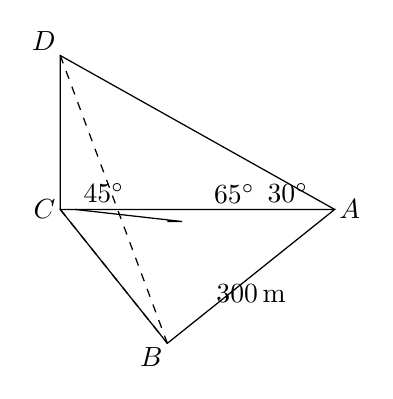
\begin{tikzpicture}[scale=0.85, line width=0.45pt,
  every node/.style={inner sep=1.5pt}]
  \coordinate (A) at (2.5,0.4);
  \coordinate (C) at (-1.6,0.4);
  \coordinate (D) at (-1.6,2.7);
  \coordinate (B) at (0.0,-1.6);
  \draw (A)--(B)--(C)--cycle;
  \draw (C)--(D)--(A);
  \draw[dashed] (C)--(B);
  \draw[dashed] (D)--(B);
  \draw (C)+(0.22,0)--(0.22,0.22)--(0,0.22);
  \node[anchor=west] at (A) {$A$};
  \node[anchor=north east] at (B) {$B$};
  \node[anchor=east] at (C) {$C$};
  \node[anchor=south east] at (D) {$D$};
  \node at (1.8,0.65) {$30^\circ$};
  \node at (1.0,0.63) {$65^\circ$};
  \node at (-0.95,0.65) {$45^\circ$};
  \node[anchor=north] at (1.25,-0.65) {$300\,\mathrm m$};
\end{tikzpicture}
\end{center}
\nopagebreak[4]
\Needspace{4\baselineskip}
\textbf{解析}

\Needspace{5\baselineskip}
设山脚为 $C$、山顶为 $D$。由方位条件，在三角形 $ABC$ 中
\nopagebreak[4]
\[
\angle ACB=45^\circ,
\qquad \angle CAB=65^\circ,
\qquad \angle ABC=70^\circ,
\qquad AB=300\text{ 米}.
\]
\Needspace{5\baselineskip}
由正弦定理，
\nopagebreak[4]
\[
AC=\frac{AB\sin70^\circ}{\sin45^\circ}
=300\sqrt2\sin70^\circ\text{ 米}.
\]
\Needspace{5\baselineskip}
在直角三角形 $ACD$ 中，仰角 $\angle CAD=30^\circ$，所以
\nopagebreak[4]
\[
CD=AC\tan30^\circ
=100\sqrt6\sin70^\circ
\approx100\times2.45\times0.940
\approx230\text{ 米}.
\]
因此山高约为 $230$ 米。

\gkanswer{答案：山高约为 $230$ 米。}

\end{answer}
\begin{answer}
\gksolhead{10}{}

\textbf{题目}：

下面甲、乙两题，选作一题。

\Needspace{5\baselineskip}
甲、$k$ 是什么实数的时候，方程
\nopagebreak[4]
\[
x^2-2(k+3)x+3k^2+1=0
\]
有实数根？

\Needspace{5\baselineskip}
乙、设方程
\nopagebreak[4]
\[
8x^2-(8\sin\alpha)x+2+\cos2\alpha=0
\]
的两个根相等，求 $\alpha$。

\Needspace{4\baselineskip}
\textbf{解析}

\Needspace{5\baselineskip}
甲：方程有实数根的充要条件是判别式不小于零：
\nopagebreak[4]
\[
[-2(k+3)]^2-4(3k^2+1)\ge0.
\]
\Needspace{5\baselineskip}
化简得
\nopagebreak[4]
\[
-k^2+3k+4\ge0,
\qquad (k+1)(k-4)\le0.
\]
\Needspace{5\baselineskip}
因此
\nopagebreak[4]
\[
-1\le k\le4.
\]

\Needspace{5\baselineskip}
乙：两个根相等，故
\nopagebreak[4]
\[
(8\sin\alpha)^2-4\cdot8(2+\cos2\alpha)=0.
\]
\Needspace{5\baselineskip}
利用 $\cos2\alpha=1-2\sin^2\alpha$，得
\nopagebreak[4]
\[
4\sin^2\alpha-3=0,
\qquad \sin\alpha=\pm\frac{\sqrt3}{2}.
\]
\Needspace{5\baselineskip}
所以通解为
\nopagebreak[4]
\[
\alpha=n\pi\pm\frac\pi3,
\qquad n\in\mathbb Z.
\]

\gkanswer{答案：甲项为 $-1\le k\le4$；乙项为 $\alpha=n\pi\pm\dfrac\pi3$（$n\in\mathbb Z$）。}

\end{answer}